\section{Sobre la estructura de bandas}
\subsection{Modelo de enlace fuerte}

A bajas energías, los enlaces $ \sigma $ resultan estables y son los encargados de 
mantener la estructura del grafeno, de modo que los electrones que forman enlaces $ 
\pi $ con orbitales $ 2p_z $ son los responsables de la dinámica electrónica del 
grafeno a bajas energías, cerca del nivel de Fermi. Además, cada átomo de carbono 
aporta o tiene asociado uno de estos electrones $ \pi $ de interés.

Esto es lo que nos lleva a considerar obtener la teoría de estructura de bandas para 
el grafeno mediante un \emph{modelo de enlace fuerte}. Este procedimiento fue 
llevado a cabo por \textcite{Wallace1947} para la estructura del grafito en su 
trabajo titulado \textbf{La Teoría de Bandas del Grafito}.

El modelo de enlace fuerte, desarrollado por \textcite{Bloch1929}, se basa en 
analizar los estados de la red como la superposición  de las funciones de onda de 
cada átomo como si estuviese aislado, es por eso que la presencia de un solo 
electrón $ \pi $ asociado a cada átomo de carbono en el grafeno garantiza buenos 
resultados cualitativos.

A continuación se estudiará el modelo de enlace fuerte de manera general para redes 
compuestas \autocite[Según lo desarrollan en ][]{Grosso2000solid}, posteriormente se 
estudiará el caso particular del grafeno.


\subsection{Aproximación a la función de onda del cristal}
Para comenzar se define entonces el orbital atómico $ \ket{\phi_i(\rvect)} $ con 
números cuánticos $ i $ y una energía asociada $ E_i $ para el átomo de alguna 
sub-red centrado en una celda unitaria de referencia.
Subsecuentemente se define el orbital atómico $ \ket{\phi_{i\mu}(\rvect - \dvect{\mu})} $ 
para cada átomo con números cuánticos $ i $ y energía $ E_{i\mu} $ en posición 
$ \dvect{\mu} $ dentro de la celda unitaria.
Por último se trabaja entonces con las traslaciones discretas $ \Rvect{m} $ a otras 
celdas unitarias diferentes de la celda unitaria de referencia, indicado por 
$ \ket{\phi_{i\mu}(\rvect - \dvect{\mu} - \Rvect{m})} $ el mismo orbital para el 
átomo en la posición trasladada.

Basado en la superposición de estos orbitales se busca entonces aproximar la función 
de onda para el cristal, dicha función de onda debe cumplir el 
\emph{Teorema de Bloch} que establece que cualquier solución (físicamente aceptable) 
de la ecuación de Schrödinger en un potencial periódico toma la forma de una onda 
plana viajera modulada en la escala microscópica por una función apropiada para la 
periodicidad de la red. De modo que la función de onda aproximada es necesario 
definirla mediante una \emph{suma de Bloch} de vector de onda $ \kvect $, con factor 
de normalización $ \frac{1}{\sqrt N} $ donde $ N $ es el número de celdas de la red.
\begin{equation}\label{eq:blochsum}
\ket{\Phi_{i\mu}(\kvect, \rvect)} = \frac{1}{\sqrt N}\sum_{\Rvect{m}} e^{i\kvect\cdot\Rvect{m}} \ket{\phi_{i\mu}(\rvect - \dvect{\mu} - \Rvect{m})}
\end{equation}
Finalmente un número de sumas de Bloch (correspondientes a los orbitales atómicos 
con la misma energía o razonablemente cercanos) se utilizan como los estados base 
para describir la función de onda del cristal en la región energética seleccionada 
de interés
\begin{equation}\label{eq:crystalwave}
\ket{\psi(\kvect, \rvect)} = \sum_{i\,\mu} \ket{\Phi_{i\mu}(\kvect, \rvect)}\underbrace{\bra{\Phi_{i\mu}(\kvect, \rvect)}\ket{\psi(\kvect, \rvect)}}_{a_{i\mu}(\kvect)} = \sum_{i\,\mu} a_{i\mu}(\kvect)\ket{\Phi_{i\mu}(\kvect, \rvect)}
\end{equation}

Sin embargo, para el caso específico del grafeno cerca del nivel de Fermi como se ha 
mencionado previamente  es únicamente de nuestro interés los electrones $ \pi $ que 
se encuentran en el estado $ \ket{2p_z} $, de modo que es posible abandonar ahora el 
sub-índice $ i $ para complicar un poco menos la notación sin alejarnos de nuestro 
cometido.

\subsection{El Hamiltoniano del cristal}

La \emph{ecuación de Schrödinger} para un cristal se describe como es usual de la forma
\begin{equation}\label{eq:schroedinger}
\widehat{H}\ket{\psi(\kvect, \rvect)} = E(\kvect)\ket{\psi(\kvect, \rvect)}
\end{equation}
donde el Hamiltoniano para un electrón en la red se define como
\begin{equation}\label{eq:crystallhamiltonian}
\widehat{H} = \frac{\widehat{p}^2}{2m} + V(\rvect)
\end{equation}
donde $ \widehat{p} = \frac{\hbar}{i}\nabla $ es el operador momento y 
$ V(\rvect + \Rvect{m}) = V(\rvect) $ es el potencial periódico cristalino (es por 
esto que requeríamos en la sección anterior que la función de onda cumpliera el 
teorema de Bloch)

Para el modelo de enlace fuerte para redes compuestas se aproxima el potencial 
cristalino como la superposición de los potenciales atómicos esféricamente 
simétricos de los átomos centrados en la posición $ \dvect{mu} $ de la celda 
unitaria $ \Rvect{m} $, $ V_{a\mu}(\rvect - \dvect{\mu} - \Rvect{m}) $, tal que el 
Hamiltoniano de enlace fuerte tiene la forma
\begin{equation}\label{eq:TBHamiltonian}
\widehat{H} = \frac{\widehat{p}^2}{2m} + \sum_{\Rvect{m}\dvect{\mu}} V_{a\mu}(\rvect - \dvect{\mu} - \Rvect{m})
\end{equation}
Y, debido a que el orbital atómico $ \ket{\phi_{i\mu}(\rvect - \dvect{\mu})} $ es un 
auto-estado del Hamiltoniano atómico con auto-valor $ E_{i\mu} $, es conveniente 
escribir el Hamiltoniano de enlace fuerte como la suma del Hamiltoniano atómico más 
la superposición de los potenciales cristalinos debido al resto  de los átomos de la 
red, es decir
\begin{align}
\widehat{H} &= \underbrace{\frac{\widehat{p}^2}{2m} + V_{a\nu}(\rvect - \dvect{\nu})}_{\widehat{H}_{a\nu}} + \underbrace{\sum_{\Rvect{m}\neq0\,\dvect{\mu}}V_{a\mu}(\rvect - \dvect{\mu} - \Rvect{m})}_{V^\prime(\rvect)} \nonumber\\
\widehat{H} &= \widehat{H}_{a\nu} + V^\prime(\rvect) \label{eq:TBHamiltonianAtom}
\end{align} 

Tomando en cuenta todas estas consideraciones, ya se tienen entonces las 
herramientas para resolver la ecuación de Schrödinger cómodamente

\subsection{Resolución de la ecuación de Schrödinger}

Para comenzar a resolver la ecuación de Schrödinger se multiplica la ecuación \eqref{eq:schroedinger} por $ \bra{\psi(\kvect, \rvect)} $ por la izquierda, y se procede el desarrollo a partir de ahí

\begin{align*}
\bra{\psi}\widehat{H}\ket{\psi}(\kvect, \rvect) &= \bra{\psi}E\ket{\psi}(\kvect, \rvect) \qq{aplicando la relación \eqref{eq:crystalwave}}\\
\sum_{\mu\,\nu}
\underbrace{\bra{\psi}\ket{\Phi_{\mu}}}_{a^*_\mu}
\underbrace{\bra{\Phi_{\mu}}\widehat{H}\ket{\Phi_{\nu}}}_{\mathcal{H}_{\mu\nu}}
\underbrace{\bra{\Phi_{\nu}}\ket{\psi}}_{a_\nu}
(\kvect, \rvect) 
&= \sum_{\mu\,\nu}
\underbrace{\bra{\psi}\ket{\Phi_{\mu}}}_{a^*_\mu}
E\underbrace{\bra{\Phi_{\mu}}\ket{\Phi_{\nu}}}_{\mathcal{S}_{\mu\nu}}
\underbrace{\bra{\Phi_{\nu}}\ket{\psi}}_{a_\nu}
(\kvect, \rvect) \\
\sum_{\mu\,\nu}a^*_\mu\,\mathcal{H}_{\mu\nu}\,a_\nu (\kvect)&= \sum_{\mu\,\nu}a^*_\mu\,E\,\mathcal{S}_{\mu\nu}\,a_\nu (\kvect)\numberthis \label{eq:presecular}
\end{align*}

La matriz $ \mathcal{H} $ se le conoce como la \emph{matriz \textbf{Hamiltoniana}}, y la matriz $ \mathcal{S} $ como la \emph{matriz de \textbf{solapamiento}}, que resulta de la no-ortogonalidad de los estados base. Ambas matrices son matrices hermíticas.

Para encontrar las auto-funciones y los auto-valores del Hamiltoniano de la red 
cristalina es entonces necesario resolver la ecuación secular resultante de la 
expresión \eqref{eq:presecular}
\begin{equation}\label{eq:secular}
\|\mathcal{H}_{\mu\nu} - E\,\mathcal{S}_{\mu\nu}\|(\kvect) = 0
\end{equation}

Para ayudarnos a resolver la ecuación secular \eqref{eq:secular} se procede a 
desarrollar los elementos $ \mathcal{H}_{\mu\nu} $ de la matriz Hamiltoniana:
\begin{align*}
\mathcal{H}_{\mu\nu}(\kvect) &= \bra{\Phi_{\mu}(\kvect, \rvect)}\widehat{H}\ket{\Phi_{\nu}(\kvect, \rvect)} \qq{aplicando la relación \eqref{eq:blochsum}}\\
\mathcal{H}_{\mu\nu}(\kvect) &= \frac{1}{N} \sum_{\Rvect{m}\Rvect{n}}e^{i\kvect\cdot(\Rvect{n} - \Rvect{m})} \bra{\phi_{\mu}(\rvect - \dvect{\mu} - \Rvect{m})}\widehat{H}\ket{\phi_{\nu}(\rvect - \dvect{\nu} - \Rvect{n})}\\
\intertext{Debido a que el Hamiltoniano es traslacionalmente invariante se puede 
	establecer $ \Rvect{m} = \mathbf0 $ y la sumatoria sobre $ \Rvect{m} $ 
	equivaldría al número $ N $ de celdas de la red}
\mathcal{H}_{\mu\nu}(\kvect) &= \frac{\cancelshade N}{\cancelshade N}\sum_{\Rvect{n}}e^{i\kvect\cdot\Rvect{n}} \bra{\phi_{\mu}(\rvect - \dvect{\mu})}\widehat{H}\ket{\phi_{\nu}(\rvect - \dvect{\nu} - \Rvect{n})} \qq{sustituyendo por \eqref{eq:TBHamiltonianAtom}}\\
\mathcal{H}_{\mu\nu}(\kvect) &= \sum_{\Rvect{n}}e^{i\kvect\cdot\Rvect{n}} \bra{\phi_{\mu}(\rvect - \dvect{\mu})}\widehat{H}_{a\mu}+V^\prime(\rvect)\ket{\phi_{\nu}(\rvect - \dvect{\nu} - \Rvect{n})}\\
\begin{split}
\mathcal{H}_{\mu\nu}(\kvect) &= \sum_{\Rvect{n}}e^{i\kvect\cdot\Rvect{n}}\left[ E_\mu\bra{\phi_{\mu}(\rvect - \dvect{\mu})}\ket{\phi_{\nu}(\rvect - \dvect{\nu} - \Rvect{n})}\right.\\
&\left.\qquad\qquad\qquad\qquad+\bra{\phi_{\mu}(\rvect - \dvect{\mu})}V^\prime(\rvect)\ket{\phi_{\nu}(\rvect - \dvect{\nu} - \Rvect{n})}\right]
\end{split}
\\
\mathcal{H}_{\mu\nu}(\kvect) &=\big[E_{\mu}\bra{\Phi_{\mu}(\kvect, \rvect)}\ket{\Phi_{\nu}(\kvect, \rvect)} + \underbrace{\bra{\Phi_{\mu}(\kvect, \rvect)}V^\prime(\rvect)\ket{\Phi_{\nu}(\kvect, \rvect)}}_{\mathcal{T}_{\mu\nu}(\kvect)}\big]\\
\mathcal{H}_{\mu\nu}(\kvect) &= \bqty{E_\mu(\kvect)\,\mathcal{S}_{\mu\nu}(\kvect) + \mathcal{T}_{\mu\nu}(\kvect)} \numberthis\label{eq:HamiltonianMatrix}
\end{align*}

Donde $ \mathcal{T}(\kvect) $ se conoce como la \emph{matriz de \textbf{salto}}, 
cuyos elementos $ \mu\nu $ se componen por la sumatoria sobre $ \Rvect{n} $ del 
producto de lo que se conoce como las \emph{integrales de salto} 
\[ \bra{\phi_{\mu}(\rvect - \dvect{\mu})}V^\prime(\rvect)\ket{\phi_{\nu}(\rvect - 
	\dvect{\nu} - \Rvect{n})} \] 
por los factores de fase $ e^{i\kvect\cdot\Rvect{n}} $, similarmente se aprecia como 
la matriz de solapamiento se compone de la misma manera, con la diferencia de usar 
las \emph{integrales de solapamiento} 
\[ \bra{\phi_{\mu}(\rvect - \dvect{\mu} - \Rvect{m})}\ket{\phi_{\nu}(\rvect - 
	\dvect{\nu} - \Rvect{n})} \] 
en lugar de la integrales de salto.

La consideración fundamental del modelo de enlace fuerte implica que las 
interacciones debido átomos lejanos del átomo de estudio ($ \Rvect{n}\neq\mathbf0 $ 
e incluso $ \Rvect{n}=\mathbf0 \land \dvect{\mu}\neq\dvect{\nu} \forall \mu\neq\nu 
$) deberían ser despreciables, sin embargo en la práctica, la sumatoria sobre $ 
\Rvect{n} $ se restringe a casos determinados que fungen como correcciones al modelo 
ideal.

De modo que sustituyendo \eqref{eq:HamiltonianMatrix} en \eqref{eq:secular} la 
ecuación secular queda de la forma:
\begin{align*}
\|\bqty{E_\mu\,\mathcal{S}_{\mu\nu} + \mathcal{T}_{\mu\nu}} - E\,\mathcal{S}_{\mu\nu}\|(\kvect) &= 0 \\
\|\mathcal{T}_{\mu\nu}+\bqty{E_\mu-E}\mathcal{S}_{\mu\nu}\|(\kvect) &= 0 \\
\|\mathcal{T}_{\mu\nu}-\bqty{E-E_\mu}\mathcal{S}_{\mu\nu}\|(\kvect) &= 0 \numberthis\label{eq:workedSecular}
\end{align*}
Partiendo de aquí es posible trabajar con los casos particulares, estableciendo las 
restricciones y condiciones necesarias para cada caso.

\subsection{Caso particular: Carbono y la red de panal de abejas}

Para el caso particular del grafeno, se tiene que los vectores primitivos de la red 
recíproca que componen las traslaciones discretas $ \Rvect{n} $ son cualquier par 
definido según la Ec.\eqref{eq:avectors}, particularmente se utilizarán los vectores 
$ \avect{1} $ y  $ \avect{2} ,$ y, si centramos la celda unitaria sobre un átomo de 
la sub-red A, los vectores que definen las posiciones de los átomos dentro de la 
celda unitaria serían $ \dvect{0} = \mathbf0 $ para los átomos de la sub-red A y 
cualquiera de los 3 vectores definidos en las Ec.\eqref{eq:deltavec} para los átomos 
de la sub-red B, particularmente se utilizará el vector $ \dvect{1} $.

El hecho de que se encuentren solo dos átomos dentro de la celda unitaria (descritos 
por dos vectores $\dvect{\mu}$) implica entonces que las matrices $ \mathcal{S} $ y 
$ \mathcal{T} $ serán de dimensión $ 2\times2 $ lo cual a su vez implica la 
presencia de dos bandas relacionadas a los electrones $\pi$.

Las sumatorias de los elementos de la matriz de solapamiento $ \mathcal{S} $ se 
restringirán de modo que cubran únicamente los efectos debido a los vecinos más 
próximos (\texttt{nn}), ya que el solapamiento debido a átomos más lejanos 
(\texttt{nnn} o \texttt{nnnn}) se puede considerar despreciable.
Para la matriz de salto $ \mathcal{T} $, cuyas integrales tienen efectos de mayor 
rango, se restringirán para que cubran a los vecinos más próximos y los siguientes 
vecinos más próximos \figref{fig:nnandnnn}.

\begin{figure}[hbt]
	\Centering
	\begin{tikzpicture}[node distance=0pt]
	\begin{pgfonlayer}{foreground}
	\triangularSites[site/.default=red, graphene]{3}{4}
	\node at (triangular cs:x=2, y=1, graphene) [subAsite] (A-1-2) {};
	\triangularSites[site/.default=blue, jstart=2]{2}{4}
	\node at (triangular cs:x=0, y=1) [subBsite] {};
	\end{pgfonlayer}
	
	\useasboundingbox (current bounding box.north west) (current bounding box.south east);
	
	\begin{pgfonlayer}{background}
	\honeyLattice[site/.append style={draw=none, fill=none}]{3}{5}
	
	\draw[vectors=red] (HA-1-1) edge (HA-1-0) edge (HA-1-2)
	\foreach \i in {0,2}\foreach \j in {0,1}{edge (HA-\i-\j)};
	\draw[vectors=blue] (HA-1-1) edge (HB-0-1);
	\end{pgfonlayer}
	
	\draw[white, ultra thick] (HB-0-1) edge (HB-1-0) edge (HB-1-1);
	\draw[vectors=red] (HB-0-1) edge (HB-1-0) edge (HB-1-1);
	
	\node[red, left=of HA-0-0]  {$\avect{2}$};
	\node[red, right=of HA-0-1] {$\avect{1}$};
	\node[blue,above=of HB-0-1] {$\dvect{1}$};
	\node[red, above=of HA-1-0] {$\avect{2}-\avect{1}=-\avect{3}$};
	\node[red, above=of HA-1-2] {$\avect{1}-\avect{2}=\avect{3}$};
	\node[blue,left=of HB-1-0]  {$\dvect{1}\color{red}-\avect{1}$};
	\node[blue,right=of HB-1-1] {$\dvect{1}\color{red}-\avect{2}$};
	\node[red, left=of HA-2-0]  {$-\avect{1}$};
	\node[red, right=of HA-2-1] {$-\avect{2}$};
	\end{tikzpicture}
	\caption[Vectores \texttt{nn} y \texttt{nnn} para la red de panal de abejas]{\label{fig:nnandnnn} Vectores de interés para describir las traslaciones correspondientes a los vecinos más próximos y los siguientes vecinos más próximos con referencia a un nodo arbitrario de la red de panal de abejas.}
\end{figure}

De modo que los elementos de las matrices se expresan explícitamente de las 
siguientes formas:

\subsubsection{Matriz de solapamiento}
Los elementos fuera de la diagonal de la matriz de solapamiento se expresan como:
\begin{multline}\label{eq:Soffdiag}
\mathcal{S}_{01}(\kvect)=\mathcal{S}_{10}^*(\kvect)\approx\bra{\phi_{0}(\rvect)}\ket{\phi_{1}(\rvect - \dvect{1})} \\*+ \SnnInt{\avect{1}} \\*+ \SnnInt{\avect{2}}
\end{multline}
Es notorio que estos elementos corresponden al solapamiento con los vecinos más 
próximos y que debido a la simetría de la red, la amplitud de las integrales de 
solapamiento son iguales ($ S_{\mathtt{nn}} $), de modo que \eqref{eq:Soffdiag} se 
puede escribir como
\begin{equation}\label{eq:SoffdiagShort}
\begin{split}
\mathcal{S}_{01}(\kvect)=\mathcal{S}_{10}^*(\kvect)&\approx S_\mathtt{nn} \underbrace{\qty(1 + e^{-i\kvect\cdot\avect{1}} + e^{-i\kvect\cdot\avect{2}})}_{\alpha^*(\kvect)} \\*&\approx S_\mathtt{nn} \alpha^*(\kvect)
\end{split}
\end{equation}

Los elementos diagonales de la matriz se expresan como:
\begin{equation}\label{eq:Sdiag}
\mathcal{S}_{00}(\kvect) = \mathcal{S}_{11}(\kvect) \approx \bra{\phi_{0}(\rvect)}\ket{\phi_{0}(\rvect)} = 1
\end{equation}
Debido a la restricción según la cuál no es de nuestro interés tomar en cuenta el 
solapamiento debido a los siguientes vecinos más cercanos, los elementos diagonales 
de la matriz se componen unicamente del producto de los orbitales atómicos iguales 
que deben estar normalizados.

\subsubsection{Matriz de salto}
Los elementos fuera de la diagonal de la matriz de salto se expresan como:
\begin{multline}\label{eq:Toffdiag}
\mathcal{T}_{01}(\kvect)=\mathcal{T}_{10}^*(\kvect)\approx\bra{\phi_{0}(\rvect)}V^\prime(\rvect)\ket{\phi_{1}(\rvect - \dvect{1})} \\*+ \TnnInt{\avect{1}} \\*+ \TnnInt{\avect{2}}
\end{multline}
E igual que con la matriz de solapamiento, corresponde entonces al efecto debido los 
vecinos más cercanos y la amplitud de las integrales de salto $ T_{\mathtt{nn}} $ 
son iguales debido a la simetría de la red de modo que \eqref{eq:Toffdiag} se puede 
escribir como:
\begin{equation}\label{eq:ToffdiagShort}
\begin{split}
\mathcal{T}_{01}(\kvect)=\mathcal{T}_{10}^*(\kvect)&\approx T_\mathtt{nn} \qty(1 + e^{-i\kvect\cdot\avect{1}} + e^{-i\kvect\cdot\avect{2}}) \\*&\approx T_\mathtt{nn} \alpha^*(\kvect)
\end{split}
\end{equation}

Los elementos diagonales de la matriz se expresan como:
\begin{multline}\label{eq:Tdiag}
\mathcal{T}_{00}(\kvect)=\mathcal{T}_{11}(\kvect) \approx \bra{\phi_{0}(\rvect)}V^\prime(\rvect)\ket{\phi_{0}(\rvect)} \\*
\shoveright{+ \TnnnInt{\avect{1}} + \TnnnInt{\avect{2}}} \\*
\shoveright{+ \TnnnInt[-]{\avect{1}} + \TnnnInt[-]{\avect{2}}} \\*
\shoveright{+ \TnnnInt{(\avect{1} - \avect{2})}} \\*+
\TnnnInt[-]{(\avect{1} - \avect{2})}
\end{multline}
El primer término de \eqref{eq:Tdiag} corresponde a una energía in situ debido a 
todo el potencial de la red. En esta posición $ \Rvect{n} = \mathbf0 $ el potencial 
se debe únicamente a la contribución del átomo de carbono del sitio y $ 
V^\prime(\rvect) $ tiene su valor mínimo, de modo que su valor es despreciable.

En bajo una lógica similar a la desarrollada para los elementos fuera de la diagonal 
de las matrices $ \mathcal{S} $ y $ \mathcal{T} $, las amplitudes de las integrales 
de \eqref{eq:Tdiag} son equivalentes ($ T_{\mathtt{nnn}} $) y entonces la expresión 
se puede reescribir como:
\begin{align*}
\mathcal{T}_{00}(\kvect) &= \mathcal{T}_{11}(\kvect) \\
\mathcal{T}_{00}(\kvect) &\approx T_{\mathtt{nnn}} \Big[\foreach \sign in {,-}\foreach \av in {{\avect{1}},{\avect{2}},{(\avect{1}-\avect{2})}}{e^{\sign i\kvect\cdot\av}+} 3-3\Big]\\*
&\approx T_{\mathtt{nnn}} \bqty{\foreach \sign in {,-}{\pqty{1+e^{\sign i\kvect\cdot\avect{1}}+e^{\sign i\kvect\cdot\avect{2}}}} -3}\\*
&\approx T_{\mathtt{nnn}}\bqty{\alpha(\kvect)\alpha^*(\kvect) -3}\\*
&\approx T_{\mathtt{nnn}}\big[\abs{\alpha(\kvect)}^2 - 3\big] \numberthis\label{eq:TdiagShort}
\end{align*}

Conociendo entonces cada elemento que compone las matrices involucradas en la 
ecuación secular \eqref{eq:workedSecular} se puede proceder a resolverla, para 
obtener los valores de la energía $ E(\kvect) $

\subsection{La ecuación secular}

Antes de resolver la ecuación secular \eqref{eq:workedSecular} es necesario resaltar 
otra particularidad que se aplica a las redes de grafeno, en el cuál ambos átomos 
dentro de la celda unitaria son átomos de carbono con la misma configuración 
electrónica, de modo que el aporte de energía $ E_\nu(\kvect) $ es constante para 
cada $ \nu\in\{0,1\} $ por lo cual simplemente implica un corrimiento de todo el 
espectro energético, de modo que es posible fijar $ E_\nu(\kvect) = 0 $ como 
referencia sin perder generalidad.

Finalmente la ecuación secular, mediante los valores \eqref{eq:SoffdiagShort}, 
\eqref{eq:Sdiag}, \eqref{eq:ToffdiagShort} y \eqref{eq:TdiagShort} se presenta de la 
forma

\begin{align*}
\mdet{T_{\mathtt{nnn}}\big[\abs{\alpha(\kvect)}^2 - 3\big] - E(\kvect) & \bqty{T_\mathtt{nn}-E(\kvect)S_\mathtt{nn}} \alpha^*(\kvect) \\ \bqty{T_\mathtt{nn}-E(\kvect)S_\mathtt{nn}} \alpha(\kvect) & T_{\mathtt{nnn}}\big[\abs{\alpha(\kvect)}^2 - 3\big] - E(\kvect)} &= 0\\
\Bqty{T_{\mathtt{nnn}}\big[\abs{\alpha(\kvect)}^2 - 3\big] - E(\kvect)}^2 - \bqty{T_\mathtt{nn}-E(\kvect)S_\mathtt{nn}}^2 \abs{\alpha(\kvect)}^2 &=0
\end{align*}
Despejando
\begin{align*}
T_{\mathtt{nnn}}\big[\abs{\alpha(\kvect)}^2 - 3\big] - E(\kvect) &= \pm\bqty{T_\mathtt{nn}-E(\kvect)S_\mathtt{nn}}\abs{\alpha(\kvect)}\\
\pm E(\kvect)S_{\mathtt{nn}}\abs{\alpha(\kvect)} - E(\kvect) &= \pm T_{\mathtt{nn}}\abs{\alpha(\kvect)} - T_{\mathtt{nnn}}\big[\abs{\alpha(\kvect)}^2 - 3\big] \\
E(\kvect)\bqty{\pm S_{\mathtt{nn}}\abs{\alpha(\kvect)} - 1} &= \pm T_{\mathtt{nn}}\abs{\alpha(\kvect)} - T_{\mathtt{nnn}}\abs{\alpha(\kvect)}^2 + 3T_{\mathtt{nnn}}\\
E(\kvect) &= \frac{\pm T_{\mathtt{nn}}\abs{\alpha(\kvect)} - T_{\mathtt{nnn}}\abs{\alpha(\kvect)}^2 + 3T_{\mathtt{nnn}}}{\pm S_{\mathtt{nn}}\abs{\alpha(\kvect)} - 1}\\
\shortintertext{Definiendo $ \lambda=\mp $}
E_\lambda(\kvect) &= \frac{\lambda T_{\mathtt{nn}}\abs{\alpha(\kvect)} + T_{\mathtt{nnn}}\abs{\alpha(\kvect)}^2 - 3T_{\mathtt{nnn}}}{1+\lambda S_{\mathtt{nn}}\abs{\alpha(\kvect)}} \numberthis\label{eq:eigenEnergies}
\end{align*}

Estos son los auto-valores de la energía para el modelo de función de onda, 
auto-estados del operador Hamiltoniano, mediante estos valores es posible entonces 
desarrollar la estructura de bandas del grafeno cerca del nivel de Fermi, a 
continuación tomaremos algunas consideraciones para poder estudiarlo de manera 
cualitativa.

\subsection{La estructura de bandas y los valles de Dirac}

Para estudiar la estructura de bandas procedemos a reescribir la expresión \eqref{eq:eigenEnergies}

\begin{align*}
E_\lambda(\kvect) &= \frac{\lambda T_{\mathtt{nn}}\abs{\alpha(\kvect)} + T_{\mathtt{nnn}}\abs{\alpha(\kvect)}^2 - 3T_{\mathtt{nnn}}}{1+\lambda S_{\mathtt{nn}}\abs{\alpha(\kvect)}} \cdot \frac{1-\lambda S_{\mathtt{nn}}\abs{\alpha(\kvect)}}{1-\lambda S_{\mathtt{nn}}\abs{\alpha(\kvect)}} \\
E_\lambda(\kvect) &= \frac{\pqty{\lambda T_{\mathtt{nn}}\abs{\alpha(\kvect)} + T_{\mathtt{nnn}}\abs{\alpha(\kvect)}^2 - 3T_{\mathtt{nnn}}}\pqty{1-\lambda S_{\mathtt{nn}}\abs{\alpha(\kvect)}}}{1- S_{\mathtt{nn}}^2\abs{\alpha(\kvect)}^2}\\
\intertext{Apegándose al modelo de enlace fuerte, no sería incorrecto asumir que $S_{\mathtt{nn}}^2\lll1$ y por ende aproximar la resta en el denominador a $ 1 $.}
\intertext{De forma similar no sería alejado asumir que $T_{\mathtt{nnn}}\ll1$, lo cuál permite omitir el término $- 3T_{\mathtt{nnn}}$.}
\intertext{Las presentes aproximaciones permiten simplificar el cálculo siguiente sin perder su valor cualitativo.}
E_\lambda(\kvect) &\approx \pqty{\lambda T_{\mathtt{nn}}\abs{\alpha(\kvect)} + {T_{\mathtt{nnn}}}\abs{\alpha(\kvect)}^2}\pqty{1-\lambda S_{\mathtt{nn}}\abs{\alpha(\kvect)}}\\
E_\lambda(\kvect) &\approx \lambda T_{\mathtt{nn}}\abs{\alpha(\kvect)} - T_{\mathtt{nn}}S_{\mathtt{nn}}\abs{\alpha(\kvect)}^2 + {T_{\mathtt{nnn}}}\abs{\alpha(\kvect)}^2 - \lambda{T_{\mathtt{nnn}}}S_{\mathtt{nn}}\abs{\alpha(\kvect)}^3\\
\intertext{Como $T_{\mathtt{nnn}}<1$ y $S_{\mathtt{nn}}\ll1$ entonces $T_{\mathtt{nnn}}S_{\mathtt{nn}}\lll1$}
E_\lambda(\kvect) &\approx \lambda T_{\mathtt{nn}}\abs{\alpha(\kvect)} + T_{\mathtt{nnn}}'\abs{\alpha(\kvect)}^2 \numberthis\label{eq:firstapprox}
\end{align*}
Donde $ T_{\mathtt{nnn}}' \equiv T_{\mathtt{nnn}} - T_{\mathtt{nn}}S_{\mathtt{nn}} $ 
es equivalente a una amplitud efectiva de la matriz de salto de los segundos vecinos.

El siguiente paso concierne a expandir $ \abs{\alpha(\kvect)} $ a una forma más 
sencilla de utilizar; basado en el procedimiento en que aparece por primera vez 
\eqref{eq:TdiagShort}, se tiene que:

\begin{align*}
\abs{\alpha(\kvect)}^2 &= 3\foreach \i in {1,2,3}\foreach \sign in {,-}{+e^{\sign i\kvect\cdot\avect\i}} \\
\abs{\alpha(\kvect)}^2 &= 3\foreach \i in {1,2,3}{+2\cos(\kvect\cdot\avect\i)}\\*
\intertext{Recordando los valores $ \avect{i} $ según \eqref{eq:avectors} y 
	asumiendo que $ \kvect=\sbmqty{k_x\\k_y} $, entonces:}
%\begin{split}
\abs{\alpha(\kvect)}^2 &= 3 + 2\cos(\tfrac{a\sqrt3}{2}(k_x+\sqrt3k_y)) + 2\cos(\tfrac{a\sqrt3}{2}(-k_x+\sqrt3k_y)) %\\&
+ 2\cos(a\sqrt3k_x)
%\end{split}
\\
\abs{\alpha(\kvect)}^2 &= 1 + 4\cos(\tfrac{a\sqrt3}{2}k_x)\cos(\tfrac{3a}{2}k_y) + 4\cos[2](\tfrac{a\sqrt3}{2}k_x)\\
\abs{\alpha(\kvect)}^2 &= 1 + 4\cos(\tfrac{a\sqrt3}{2}k_x)\bqty{\cos(\tfrac{3a}{2}k_y) + \cos(\tfrac{a\sqrt3}{2}k_x)} \numberthis\label{eq:phasefactmodsqr}
\end{align*}

De modo que se sustituye la expresión del módulo del la suma de los factores de fase 
\eqref{eq:phasefactmodsqr} en la expresión \eqref{eq:firstapprox} para obtener 
finalmente el comportamiento de los niveles energéticos del cristal, cuya gráfica se 
observa en la \figref{fig:BandGraphs} para un factor (justificado por cálculos 
numéricos más robustos) de $ \frac{T_{\mathtt{nnn}}'}{T_{\mathtt{nn}}} = 0.1 $.
\begin{figure}[p]
	\Centering
	\subcaptionbox[Estructura de bandas]{Gráfico de las bandas energéticas $ E_\lambda(\kvect) $ con $ \lambda=+ $ (superior, banda de conducción) y $ \lambda=- $ (inferior, banda de valencia).}[0.65\textwidth]{
		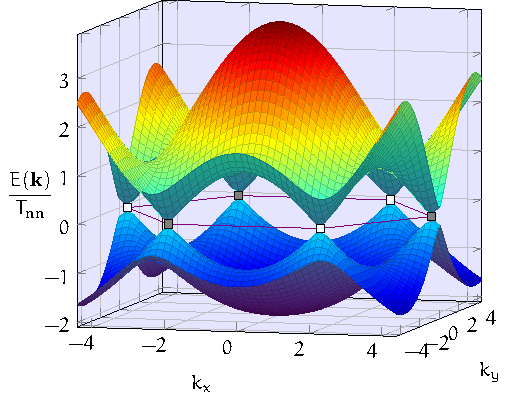
\includegraphics{./img/BandGraph.pdf}
	}\\
	\subcaptionbox[Detalle alrededor de un punto de Dirac]{Detalle alrededor de un punto de Dirac. Se observa la ausencia de una brecha energética entre las bandas, además de la forma de valle o cono de las mismas.\label{fig:diracVicinity}}[0.65\textwidth]{
		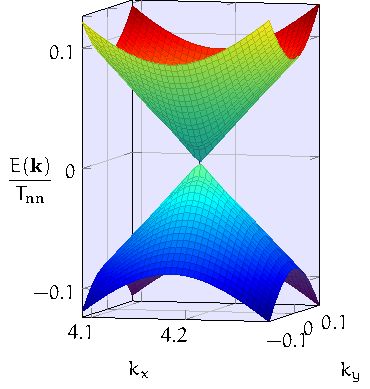
\includegraphics{./img/DiracValley.pdf}
	}
\caption{\label{fig:BandGraphs}Gráficos de la dispersión energética para los electrones $ \pi $ en el grafeno.}
\end{figure}

Debido a que cada átomo de carbono aporta únicamente un electrón $ \pi $ y cada 
electrón puede ocupar exclusivamente un estado de espín arriba o espín abajo, la 
banda baja $ \lambda=- $ se encuentra completamente llena de electrones (banda de 
valencia $ \pi $) y la banda alta $ \lambda=+ $ completamente vacía, o llena de 
huecos (banda de conducción $ \pi* $). De modo que el nivel de Fermi se ubica 
justamente donde las bandas se tocan entre sí.

Es interesante resaltar como las bandas no son simétricas, es decir que no presentan 
una simetría electrón-hueco, la cuál sí se presentaría para el caso en que $ 
T_{\mathtt{nnn}}' = 0 $ en la expresión \eqref{eq:firstapprox}, es decir que las 
correcciones de solapamiento \texttt{nn} y salto \texttt{nnn} son las responsables 
de que se presente este fenómeno.

Los puntos en los que las bandas coinciden se conocen como \emph{Puntos de Dirac} ($ 
D $) y se sitúan donde la dispersión energética \eqref{eq:firstapprox} es igual a 
cero $ E_\lambda(\kvect) = 0 $, lo cual implica que el factor de fase y por ende su 
módulo (y su módulo cuadrado) sean a su vez nulos.
\begin{align*}
	\abs{\alpha\qty(\vector{K^{D}})}^2 = 0 &= 1 + 4\cos(\tfrac{a\sqrt3}{2}k_x^D)\cos(\tfrac{3a}{2}k_y^D) + 4\cos[2](\tfrac{a\sqrt3}{2}k_x^D) \\
	\intertext{Para obtener una solución, escogemos el caso particular $ k_y^D = 0 $}
	\abs{\alpha\qty(\vector{K^{D}})}^2 = 0 &= 1 + 4\cos(\tfrac{a\sqrt3}{2}k_x^D) + 4\cos[2](\tfrac{a\sqrt3}{2}k_x^D) \\
	\abs{\alpha\qty(\vector{K^{D}})}^2 = 0 &= \bqty{1 + 2\cos(\tfrac{a\sqrt3}{2}k_x^D)}^2 \\ 
	\abs{\alpha\qty(\vector{k^{D}})} = 0 &= 1 + 2\cos(\tfrac{a\sqrt3}{2}k_x^D)
\end{align*}
\begin{equation*}
	\therefore -\frac{1}{2} = \cos(\tfrac{a\sqrt3}{2}k_x^D) \\
\end{equation*}
\begin{align*}
	\therefore
	\frac{a\sqrt3}{2}k_x^D &= \pm \frac{2\pi}{3} \\ 
	k_x^D &= \pm \frac{4\pi}{a3\sqrt3}
\end{align*}
\begin{equation}\label{eq:diracPoints}
\therefore \pm\vector{K^{D}} = \pm \frac{4\pi}{a3\sqrt3} \begin{bmatrix} 1 \\ 0 \end{bmatrix}
\end{equation}

De modo que existen dos inequivalentes Puntos de Dirac, $ D $ y $ D' $, que 
corresponden con los puntos cristalográficos $ K $ y $ K' $ \eqref{eq:KK'}. Es 
importante resaltar que estos puntos, aunque situados en el mismo lugar, son 
conceptualmente distintos.

Las bandas $ \pi $ y $ \pi* $ en la vecindad de estos puntos presentan una forma 
aproximable a conos, donde el cambio en la energía respecto a $ \kvect $ es lineal. 
Es debido a esto que se conocen como \emph{Valles de Dirac}. La asociación de esta 
región con Dirac viene dada ya que la aproximación lineal de la relación de 
dispersión alrededor de estos puntos, es similar a la descrita por la ecuación de 
Dirac para fermiones no-masivos (también conocida como la ecuación de Weyl).